\documentclass[a4paper, 11pt]{article}
\usepackage[utf8]{inputenc}
\usepackage{graphicx}
\usepackage{url}
\usepackage{caption}
\usepackage{float}
\usepackage{subcaption}

\title{\textbf{Distributed Artificial Intelligence and Intelligent Agents Project}}
\author{KTH Royal Institute of Technology \\ 
		School of Information and Communication Technology \\
		Student:Fanti Machmount Al Samisti (fmas@kth.se) \\
		Student:August Bonds (bonds@kth.se)}

\begin{document}
	
\maketitle

\tableofcontents

\section{Task 1 - GAIIA}

\subsection{Requirements Statement}

General Commonality Requirements
\begin{itemize}
\item The curators and artifact manager should be fault tolerant
\item 
\end{itemize}

Self-Optimization Commonality Requirements
\begin{itemize}
\item The curator should only bid on profitable auctions.
\item The curator should minimize the processing on every profiler query.
\item The artifact manager should adapt the price setting and price reductions to the demand and item quality.
\item The profiler should optimize bidding strategy according to client interests.
\item The artifact manager should post multiple auctions if demand is high. 
\item The artifact manager should post more low-quality items for a high price if multiple items go unsold. 
\end{itemize}

Self-Healing Commonality Requirements
\begin{itemize}
\item If there is a database corruption, artist manager should renegotiate with curators. 
\end{itemize}

Self-Protection Commonality Requirements
\begin{itemize}
\item The artist manager should detect collusions and increase the minimum price.
\item Every transaction should be atomic and persistent.
\end{itemize}

Miscellaneous Commonality Requirements
\begin{itemize}
\item bla
\end{itemize}

\subsection{Roles model}

\begin{table}[H]
	\label{my-label}
	\begin{tabular}{l p{7cm}}
		\hline
		Role Schema              & Tourist \\
		\hline
		Description              & Requests a tour based on the tourists' interests \\
		Protocols and Activities & \textbf{protocols} FIPA.Request, \textbf{activities} parse and store the reply with the artifacts, initiate a tour as soon as the reply from the curators is parsed \\
		Permissions              & \textbf{reads} available curators from \textit{DF}, \textbf{reads} tourists' interests, \textbf{changes} local artifact information \\
		\hline
		Responsibilities         &                   \\
		Liveness                 & \(Tourist=(\underline{RequestTour}.StartTour)^\omega \) \\
		Safety                   & \(interests > 0 \) \\
		\hline
	\end{tabular}
\end{table}

\begin{table}[H]
	\label{my-label}
	\begin{tabular}{l p{7cm}}
		\hline
		Role Schema              & Gallery monitoring \\
		\hline
		Description              & Monitor the artifacts database, perform maintenance tasks on it and reply to tour requests \\
		Protocols and Activities & \textbf{protocols} Fipa.INFORM, \textbf{activities} perform maintenance tasks on the artifact DB on a regular basis, monitor for problems on artifact DB \\
		Permissions              & \textbf{changes} artifact database, \textbf{reads} artifact database \\
		\hline
		Responsibilities         &                   \\
		Liveness                 & \(Monitor=\underline{Reply}\star||\underline{MaintainDB}^\omega \) \\
		Safety                   & \(databaseIntegrity \& noOfRequests < 30 \) \\
		\hline
	\end{tabular}
\end{table}

\begin{table}[H]
	\label{my-label}
	\begin{tabular}{l p{7cm}}
		\hline
		Role Schema              & Bidder \\
		\hline
		Description              & Participate in an ongoing auction \\
		Protocols and Activities & \textbf{protocols} Dutch Auction, \textbf{activities} decide on whether to bid according to his strategies \\
		Permissions              & \textbf{reads} artifact price \\
		\hline
		Responsibilities         &                   \\
		Liveness                 & \(Bidder=\underline{BidInAuction}^\omega \) \\
		Safety                   & \(interestedInAuctionedItem \) \\
		\hline
	\end{tabular}
\end{table}

\begin{table}[H]
	\label{my-label}
	\begin{tabular}{l p{7cm}}
		\hline
		Role Schema              & Artifact adder/updater \\
		\hline
		Description              & Add in the database or update an item with a newly bought artifact from the auction \\
		Protocols and Activities & \textbf{activities} add new items to the artifact DB \\
		Permissions              & \textbf{changes} artifact database, \textbf{reads} artifact database \\
		\hline
		Responsibilities         &                   \\
		Liveness                 & \(Adder=(WaitForItem.\underline{AddInDB})^\omega \) \\
		Safety                   & \(\forall itemInDatabase = unique \) \\
		\hline
	\end{tabular}
\end{table}

\begin{table}[H]
	\label{my-label}
	\begin{tabular}{l p{7cm}}
		\hline
		Role Schema              & Auction Initiator \\
		\hline
		Description              & Start and coordinate a new auction \\
		Protocols and Activities & \textbf{protocol} Dutch Auction, \textbf{activities} decide the price of the next item to be auctioned based on its earnings and strategies \\
		Permissions              & \textbf{reads} artifacts for auction, \textbf{changes} available artifacts for auction \\
		\hline
		Responsibilities         &                   \\
		Liveness                 & \(Initiator=(\underline{ChooseItemAndPrice}.GetBidders.Inform)^\omega \) \\
		Safety                   & \(auctionProfit > 0  \) \\
		\hline
	\end{tabular}
\end{table}

\subsection{Interaction model}

\subsubsection{Tour}

\begin{figure}[H]
	\caption{Tour interaction between a Tourist and one of the GalleryMonitors}
	\centering
	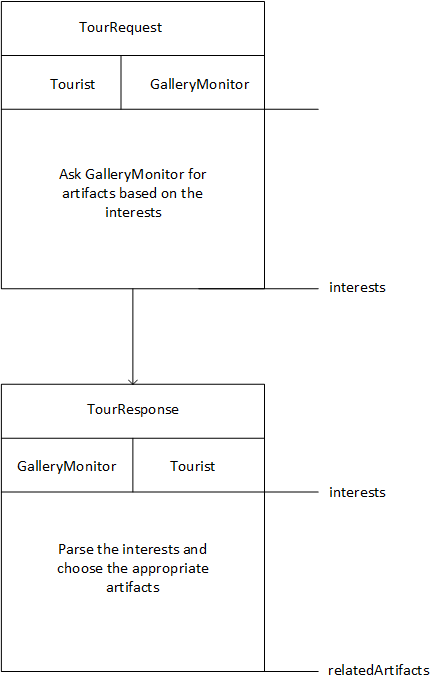
\includegraphics[scale=0.8]{./images/interaction-tourguide.png}
\end{figure}

\begin{figure}[H]
	\caption{Auction initiation: If the bidder wont participate, this interaction ends here.}
	\centering
	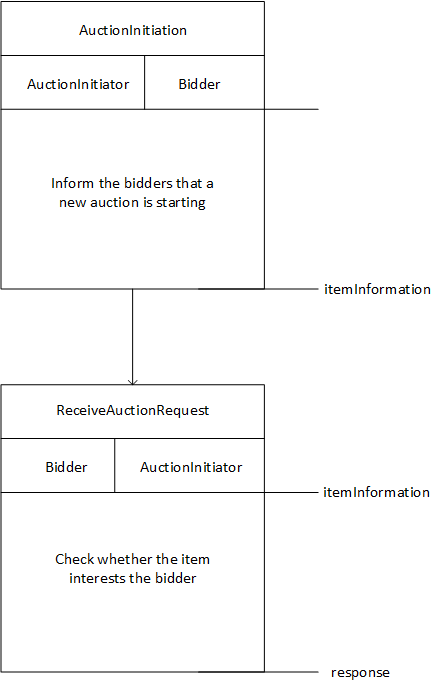
\includegraphics[scale=0.8]{./images/interaction-auction-init.png}
\end{figure}

\begin{figure}[H]
	\caption{Start an auction and the bidders decide if to bid or not}
	\centering
	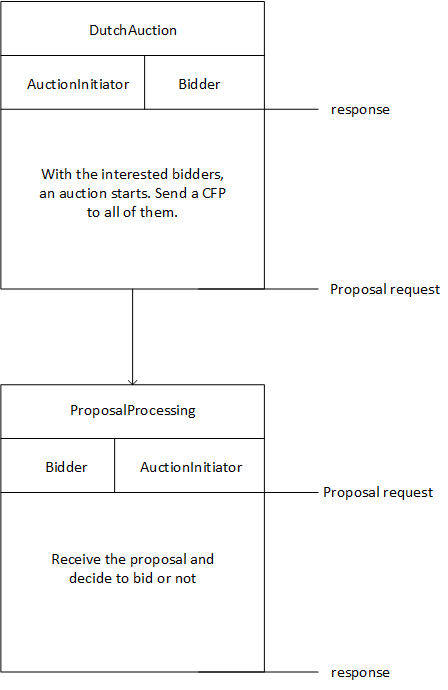
\includegraphics[scale=0.8]{./images/interaction-cfp.png}
\end{figure}

\subsection{Agent model}

\begin{figure}[H]
	\caption{Actors and their relation to the roles}
	\centering
	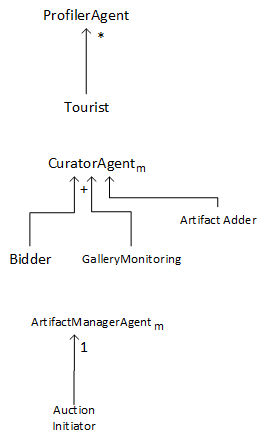
\includegraphics[scale=0.8]{./images/agent.png}
\end{figure}

\subsection{Service model}

\begin{table}[H]
	\centering
	\caption{}
	\label{my-label}
	\begin{tabular}{lllll}
		\hline
		Service & Inputs & Outputs & Pre-condition & Post-condition \\ \hline
		proposeTour & interests & artifact list & interests \textgreater 0 & profiler has a tour \\
		startAuction & \begin{tabular}[c]{@{}l@{}}available-\\ Artifacts\end{tabular} & itemToAuction & \begin{tabular}[c]{@{}l@{}}available-\\ Artifacts \textgreater 0\end{tabular} & true \\
		\begin{tabular}[c]{@{}l@{}}complete-\\ Auction\end{tabular} & bidders, item & outcome & bidders \textgreater 0 & winner $\lor$ low price \\
		bid & item & decision & true & bid $\lor$ reject proposal \\ \hline
	\end{tabular}
\end{table}

\subsection{Acquaintance model}

\begin{figure}[H]
	\caption{Actors and their communication}
	\centering
	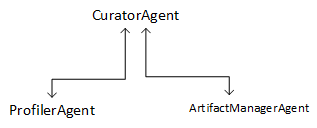
\includegraphics[scale=0.8]{./images/acquaintance.png}
\end{figure}

\subsection{Mobility model}

\begin{table}[H]
	\centering
	\caption{All places that tourists can visit and auctions can take place}
	\label{my-label}
	\begin{tabular}{lll}
		\hline
		Place Types                                                     & Description                                                                                                                                                                                                           & Instances \\ \hline
		\begin{tabular}[c]{@{}l@{}}museo galileo\\ museum\end{tabular}  & \begin{tabular}[c]{@{}l@{}}A place to see items that comprise a major \\ collection of scientific instruments. Also auctions \\ for relevant artifacts happen to enrich the collection \\ of the museum.\end{tabular} & 1         \\
		\begin{tabular}[c]{@{}l@{}}Heritage Malta\\ museum\end{tabular} & \begin{tabular}[c]{@{}l@{}}A place to see items that are protected by Maltese \\ national agency for museums. Also auctions for relevant\\ artifacts happen to enrich the collection of the museum.\end{tabular}      & 1         \\ \hline
	\end{tabular}
\end{table}

\begin{table}[H]
	\centering
	\caption{Agents and their relationship to the places}
	\label{my-label}
	\begin{tabular}{llll}
		\hline
		Agent Types & Mobile & Place Types & Constraints \\ \hline
		PrrofilerAgent & - & - & - \\
		CuratorAgent & $\surd$ & All & 1 in each place \\
		\begin{tabular}[c]{@{}l@{}}ArtifactManager\\ Agent\end{tabular} & $\surd$ & All & 1 in each place \\ \hline
	\end{tabular}
\end{table}

\begin{figure}[H]
	\caption{Actor-Place cardinality}
	\centering
	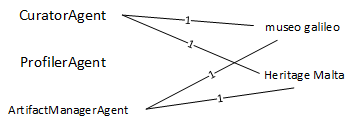
\includegraphics[scale=0.8]{./images/cardinality.png}
\end{figure}

\begin{table}[H]
	\centering
	\caption{Curator path description}
	\label{my-label}
	\begin{tabular}{ll}
		\hline
		Agent & CuratorAgent \\ \hline
		Description & \begin{tabular}[c]{@{}l@{}}An interested curator will move to a museum place\\ to take part in the auction that its been held there.\end{tabular} \\
		Origin & Any musuem in the world \\
		Destination & museo galileo or heritage malta \\
		\begin{tabular}[c]{@{}l@{}}Atomic \\ movements\end{tabular} & Move from the original museum to the destination \\
		Paths & (Original Museum - Destination - Original Museum)* \\
		\hline
	\end{tabular}
\end{table}

\begin{table}[H]
	\centering
	\caption{ArtifactManager path description}
	\label{my-label}
	\begin{tabular}{ll}
		\hline
		Agent & ArtifactManagerAgent \\ \hline
		Description & \begin{tabular}[c]{@{}l@{}}An artifact manager will move to a museum place\\ to organize the auction that its been held there.\end{tabular} \\
		Origin & Any musuem in the world \\
		Destination & museo galileo or heritage malta \\
		\begin{tabular}[c]{@{}l@{}}Atomic \\ movements\end{tabular} & Move from the original museum to the destination \\
		Paths & (Original Museum - Destination - Original Museum)* \\
		\hline
	\end{tabular}
\end{table}

\section{Task 2 - AgentUML}

\begin{figure}[H]
	\caption{Tour package and the sequence of actions to get a tour}
	\centering
	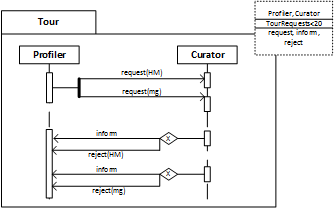
\includegraphics[scale=1]{./images/sequence-tour.png}
\end{figure}

\begin{figure}[H]
	\caption{Dutch Auction Sequence diagram}
	\centering
	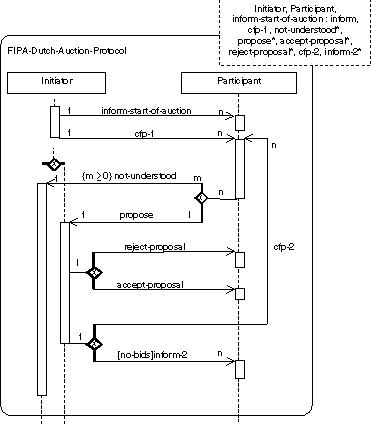
\includegraphics[scale=0.9]{./images/sequence-dutchauction.png}
\end{figure}

\begin{figure}[H]
	\caption{Profiler State-chart diagram}
	\centering
	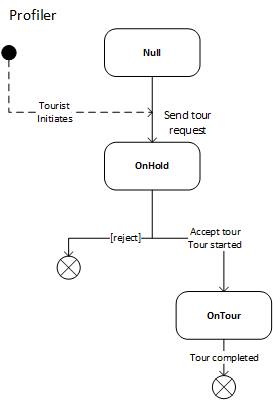
\includegraphics[scale=0.9]{./images/profilerUML.jpg}
\end{figure}
\begin{figure}[H]
	\caption{Curator State-chart diagram}
	\centering
	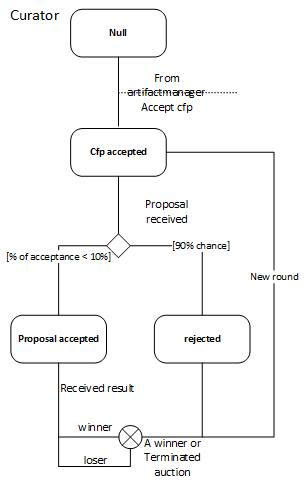
\includegraphics[scale=0.9]{./images/curatorUML.jpg}
\end{figure}
\begin{figure}[H]
	\caption{Curator State-chart diagram 2}
	\centering
	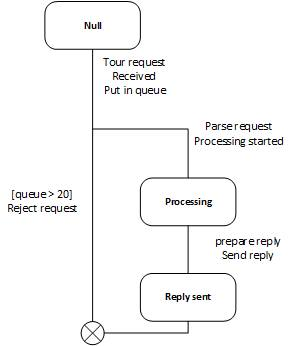
\includegraphics[scale=0.9]{./images/curator2UML.jpg}
\end{figure}
\begin{figure}[H]
	\caption{ArtifactManagement State-chart diagram}
	\centering
	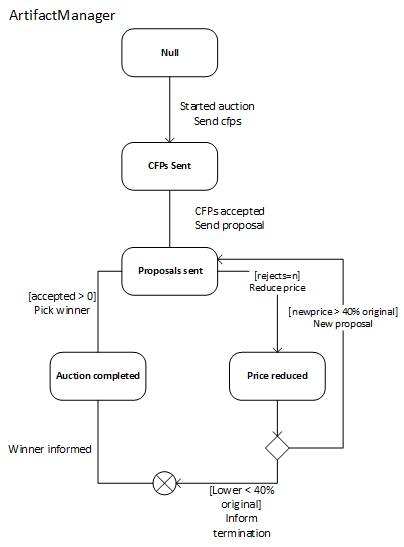
\includegraphics[scale=0.9]{./images/artifactmanagerUML.jpg}
\end{figure}
\section{Task 3 - UML and Behaviours}
\subsection{Class diagrams}

\begin{figure}[H]
	\caption{Supposed to be a class diagram}
	\centering
	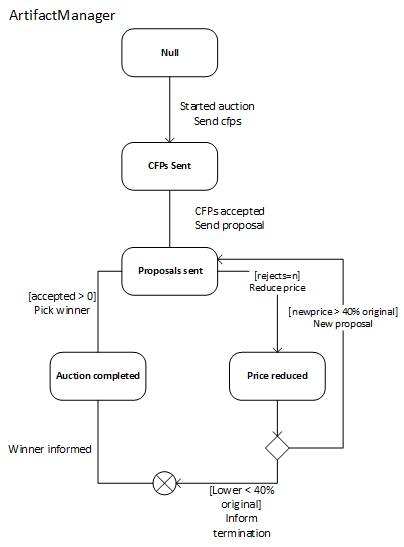
\includegraphics[scale=0.9]{./images/artifactmanagerUML.jpg}
\end{figure}

\section{Task 4 - ROMAS}
\begin{enumerate}
\item Capture use cases
\item Identify roles from use cases;
\item Construct role organization
\item For each role, if the approrpate agent does not exist, then go to (5); else
\begin{enumerate}
\item Bind roles to agents
\item Describe dynamic properties of bind relation between agents and roles
\item Go to (6)
\end{enumerate}
\item Generate agents according to roles; Go to(4). a).
\item Generate code for agents with roles bound
\end{enumerate}
\subsection{Capture Use-cases}
\begin{figure}[H]
	\caption{ROMAS Identified Use Cases}
	\centering
	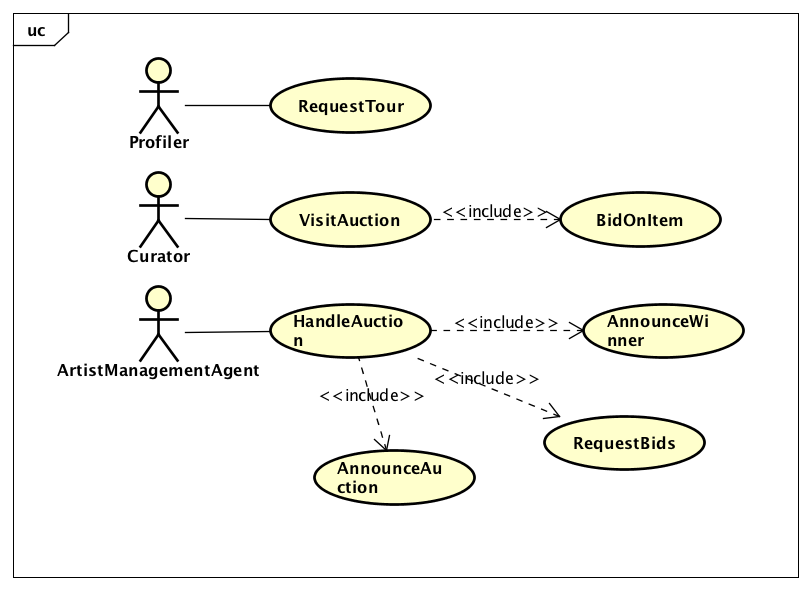
\includegraphics[width=\textwidth]{./images/ROMASusecases.png}
\end{figure}

\subsection{Identify Roles from Use-cases}
The only really important roles discovered are:
\begin{itemize}
\item Auctioneer - Person selling an item and arranging the auction
\item Buyer - Person who takes part in an auction
\item Visitor - Person who visits exhibitions (requests tours)
\end{itemize}
\subsection{Construct Role Organization}
\begin{figure}[H]
	\caption{ROMAS Role Organization}
	\centering
	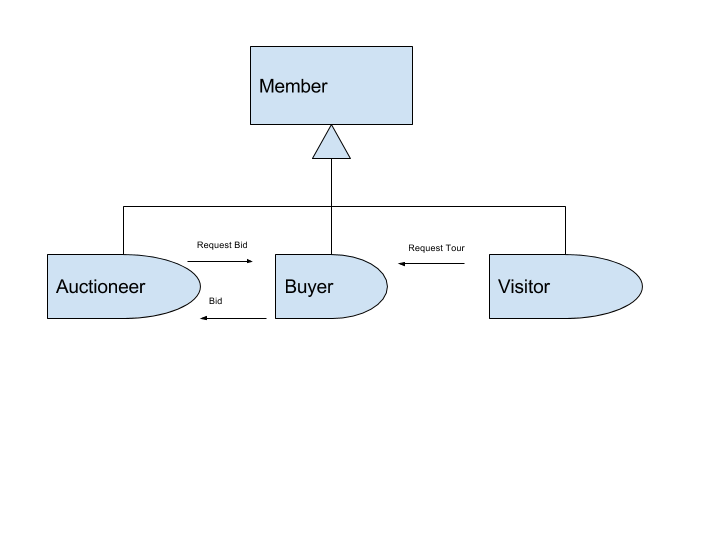
\includegraphics[width=\textwidth]{./images/ROMASroleorganization.png}
\end{figure}

Each role corresponds to an agent: Auctioneer - ArtistManagementAgent, Buyer - CuratorAgent,
Visitor - ProfilerAgent.

Because of this one-to-one relationship between agents and roles, the role automata are all
trivial.

\section{Task 5 - Framework comparison}

https://en.wikipedia.org/wiki/FIPA \\
Options(Choose 2) \\
Looks too corporate-y - http://www.agent-software.com.au/products/jack/ \\
JIAC - IJava framework - http://repositories.dai-labor.de/sites/jiactng/5.1.5/ \\
SPADE - Python framework - https://github.com/javipalanca/spade \\
JADEX - https://www.activecomponents.org/bin/view/About/Features \\

My choice would be the SPADE and JADEX. \\

We have to compare:
\begin{itemize}
	\item Architecture of platform
	\item Services provided by it
	\item Comparison of implementaBon of a simple scenario	same as	Question 2 (i.e.	Service Implementation,	Service	Registration and Service Discovery)
	\item Notable projects using it
	\item Personal opinion on practical issues compared to JADE, we could use point 3 as a starting point.
\end{itemize}

\textbf{FIPA compliance}: 
\begin{itemize}
	\item Agent Communication Channel(ACC): A mechanism which allows the platform and the agents in it to communicate with each other.
	\item Agent Management System(AMS): A way for the agents to be registered in the platform and be reachable for contact.
	\item Directory Facilitator(DF): Agents have the ability to publish services they offer, essentially yellow pages.
	\item Agent Communication Language(ACL): Common agent language, two possible syntaxes XML or Lisp based.
\end{itemize}

\subsection{SPADE}

Agent platform based on XMPP and Jabber. User(agent) and Server(platform). Agents can be in any programming language if they conform to XMPP protocol.

\textbf{XMPP}: XML inspired protocol for instant messaging and presence information. Jabber protocol at its core follows XMPP. It is an open standard and extensible. Noteable uses: Pidgin, Google Talk, iChat. \\
Features: \\
\begin{itemize}
	\item Open, public, free
	\item Asynchronous: If user online guarantee of delivery, if offline store and forward message until the client reconnects. Ease of talking with non-human systems.
	\item Decentralized: Anyone can have a server, in fact its a server network, choice of whether to trust a server.
	\item Secure
	\item Extensible
	\item Flexible: XML messaging based tech has a myriad of uses, IM is just one of them. Jabber applications beyond IM include network management, content syndication, collaboration tools, file sharing, gaming, remote systems monitoring and, now, agent communication.
\end{itemize}

\textbf{SPADE Agent Library}\\
Module to build SPADE agents that work with the SPADE Agent Platform.

\textbf{SPADE Agent Model}\\
Composed of a connection mechanism to the platform, a message dispatcher and a set of agent behaviors. Each agent is recognized by a JID(Jabber ID) that looks like (name@host, password) and by an address(xmpp://acc.myprovider.com). Each agent registers to the server as a jabber user(mandatory, not like DF in JADE) which opens a longlived communication stream. \\
A message dispatcher is responsible for receiving, delivering to a behavior queue(MessageTemplate) and sending messages. \\
Simultaneous behaviors: Cyclic, OneShot, Periodic, TimeOut, FSM and Event. \\
Message sending: like JADE \\
A SPADE agent cannot send nor receive messages until its behaviours are active. That is, do NOT place calls to the send or \_receive methods inside the \_setup and takeDown methods. \\
Search agent service, Modify Service(update your info in the AMS) \\
DF: same as Jade \\
FSM: same as Jade \\
Event Beh. : The main difference between an Event Behaviour and, say, a One-Shot Behaviour is that the Event Behaviour is not instanced nor is it running until the trigger event happens.\\
\textbf{The SPADE BDI Agent Model}: Belief-Desire-Intention:
\begin{itemize}
	\item Belief: knowledge
	\item Desire: goals
	\item Intention: the way the agent has decided to achieve his goals, Plans.
\end{itemize}
SPADE deviates from this by using Service Oriented Computing(SOC) together with dynamic compilation of services in SPADE, which we have called Distributed Goal Oriented Computing. \\
\textbf{SPADEs BDI model}:
\begin{itemize}
	\item Belief: Agent knowledge base, insert, delete, make queries.
	\item Goals and Desires: When an agent expresses a Goal, it means that the agents wishes to accomplish the expression contained in such Goal. When a goal is selected for accomplishment, it becomes active.
	\item Services: Method offered by the agent to the rest. Services can be composed into a sequence forming the Plans. Services have in their description both a pre-condition (P) and a post-condition (Q). The pre-condition P represents a state of knowledge that must be present in order to execute the Service. The post-condition Q represents the state of knowledge that the agent will achieve once the Service has been invoked.(Like MMSE ocl)
	\item Plans: Sequence of services to achieve the goals. Agents use plans to achieve their goals. Also they have their own Pre and Post conditions. Services composing a Plan's actions do not necessarily belong to the same agent.
\end{itemize}

\begin{verbatim}
Name = "agent@myhost.myprovider.com" . Addresses = ["xmpp://agent@myhost.myprovider.com"]
\end{verbatim}

\textbf{Knowledge base}: Prolog based \\
\begin{verbatim}
 $ agent.saveFact("MyList",[5,6,7,8])
 $ agent.getFact("MyList")
 > [5,6,7,8]
\end{verbatim}

\textbf{Plans and Services}: An agent exposes a method unlike JADE \\
\begin{verbatim}
#This is the method executed when the service is invoked
def s1_method(Value):
return {"Myoutput1":1} #the return value is a dict containing Facts in the form name:value

#Create the service profile
s = DF.Service(name="s1", owner=agent.getAID(), inputs=["Value"],outputs=["O1"],P=["Var(Value,0,Int)"],Q=["Var(O1,1,Int)"])

#Finally register the service
agent.registerService(s, s1_method)
\end{verbatim}

\begin{verbatim}
        agent.addPlan(inputs=["Value"],outputs=["O2"],P=["Var(Value,0,Int)"],Q=["Var(O2,2,Int)"], services=["s1","s2"])
\end{verbatim}

\textbf{GOALS:} \\
\begin{verbatim}
g = Goal("Var(O1,1,Int)")
$ def goalCompletedCB( goal ):
print "Goal completed!"

$ agent.saveFact("Value",0)

$ agent.setGoalCompletedCB( goalCompletedCB )

$ agent.addGoal( Goal("Var(Value,0,Int)") )
> "Goal completed!"
\end{verbatim}

\textbf{BDI}: During the agent execution, classic SPADE behaviours can coexist with the BDI model. Every time that a new Goal is introduced into the agent, it will try to achieve it looking for a Plan that fits the task. All this work happens in a completely transparent way for the user. \\
Easier to work with knowledge base than JADE and its done in a declarative way. \\

\textbf{Agent platform} \\
Like JADE we start a server that acts as the main point/base of the agents.

\subsection{JADEX}

BDI based \\


\subsection{Comparison}

\begin{itemize}
	\item - Jade does not support BDI like JADEX and SPADE, try to accomplish tasks, goals, plans
	\item - Jade and JADEX need a framework developed for them to run on, whereas SPADE runs on existing ones namely XMPP and Jabber
	\item + All 3 comply to the FIPA protocol e.g. ACL messages, performative etc
	\item + An agent is just a black box for the ones outside with the only way of communicating being via message passing
	\item 
\end{itemize}

%\begin{figure}
%	\begin{center}
%		\includegraphics[width=\textwidth]{agentclonelogic.jpg}
%		\caption{Overview of agent and clone logic }
%		\label{fig:results1}
%	\end{center}
%\end{figure}

\end{document}
